\subsection{Detalhamento da Base Mecânica}\label{sec::base_mec}
A base mecânica é composta pelos elementos de suporte, transporte e ancoragem do
robô no interior da turbina. Os elementos de suporte formam a estrutura
principal da base, que estruturam o ambiente para a montagem, movimentação e
funcionamento seguros do robô. Os elementos de transporte oferecem ao
manipulador graus de liberdade que permitem que este se posicione com facilidade
nos pontos ótimos para o processo. Estes elementos podem ser trilhos, atuadores
lineares, mancais de rolamento, atuadores rotativos, etc. Os elementos de
ancoragem são necessários para fixar o robô e a estrutura no ambiente. As
opções de ancoragem estudadas foram as bases magnéticas e solda, sendo a
primeira opção de preferência pois há menor risco de danificar o ambiente. As
etapas de detalhamento da base mecânica seguem a seguinte ordem: $1)$ investigação dos
graus de liberdade necessários; $2)$ configuração conceitual da base em função
dos graus de liberdade; $3)$ escolha do melhor conceito; $4)$ escolha e
dimensionamento dos elementos mecânicos que compõem a base; $5)$ testes.
Avaliamos até esta etapa do projeto os itens: $1$,$2$ e $3$.

Os graus de liberdade são fornecidos através de combinações de juntas
prismáticas e rotacionais, que no nosso caso irão permitir o movimento do robô
desde a escotilha até o ponto de interesse para o início do processo de
revestimento e entre as etapas de em cada região da pá.
Investigou-se primeiramente alguns conceitos baseados nos graus de liberadade 
necessários para fornecer à base do robô todos os posicionamentos necessários, 
de acordo com os estudos cinemáticos e dinâmicos descritos  nas
seções~\ref{sec::cinematica} e \ref{sec::dinamica}.
%TODO criar label para sec estudo dinamico

A análise dos conceitos estudados permite então compara-los e definir o que
melhor se adapta ao objetivo da solução. Nesta etapa incia-se o detalhamento da base
mecânica seguindo as diretrizes e requisitos mecânicos do projeto. A
estrutura deve ter capacidade de suportar os esforços dinâmicos do robô,
de forma que não haja grandes deformações elásticas e oscilações que possam
comprometer a precisão de posicionamento do efetuador do braço robótico.
Deve-se atentar também ao caráter dinâmico dos esforços, que causam vibrações
que podem resultar em esforços e deslocamentos elevados.
Assim, a fixação da estrutura da base no ambiente deve ser o mais rígida
possível, superdimensionando os elementos de ancoragem e minimizando as folgas
nos acoplamentos.

A entrada dos componentes da base é uma tarefa trabalhosa, devido ao acesso
limitado ao interior da turbina. O diâmetro de $800~mm$ da escotilha inferior
limita o tamanho e geometria dos equipamentos. Além disso, estes componentes devem ser
içados até a escotilha em uma altura de $5~m$ entre o piso no exterior do
ambiente confinado e seu interior. Assim, a modularidade dos elementos que compõe a base
é uma diretriz essencial a esse projeto. A facilidade de transporte, montagem e
desmontagem da base mecânica causará um grande impacto na praticidade e
agilidade de implementação da solução.

A seguir apresenta-se os conceitos analisados, em relação aos graus de
liberdade da base mecânica:

$\bullet$~\textbf{Base Prismática-Rotacional-Rotacional (P-R-R):}
  
  Neste conceito estudou-se a possibilidade de utilizar uma base com $3$ graus
  de liberdade: um prismático e dois rotacionais. O prismático seria composto
  por um trilho alinhado e paralelo ao eixo da turbina que transportaria o robô
  até a região próxima a pá. Uma junta rotacional e com eixo vertical orientaria
  a base nesta direção e uma junta perpedincular à primeira faria o
  posicionamento da base do robô para então iniciar o processo de revestimento.
  A figura~\ref{fig::base_prr} ilustra este conceito.
    
  \begin{figure}[h!]
   \centering
   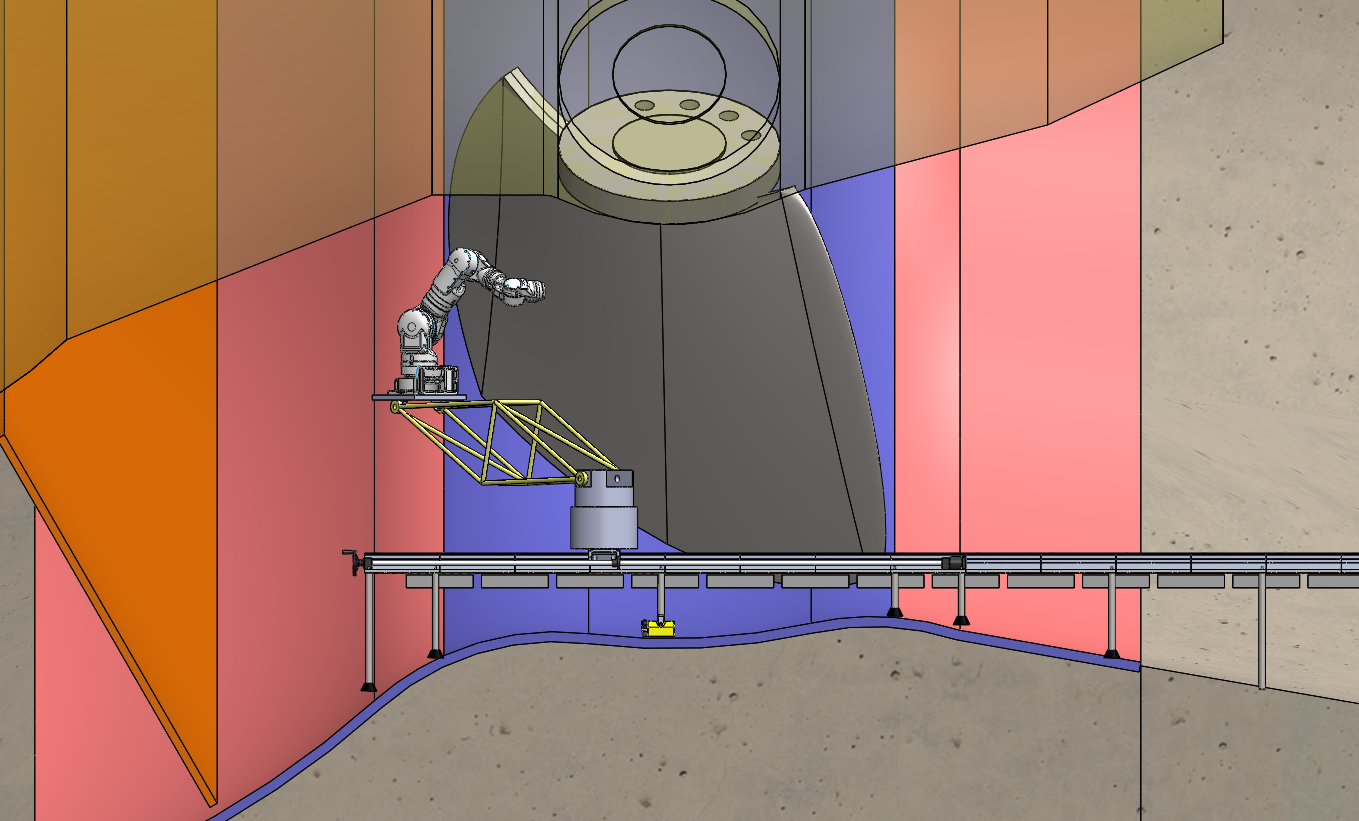
\includegraphics[width=0.8\columnwidth]{figs/bases/base_prr}
   \caption{Base Primático-Rotacional-Rotacional}
   \label{fig::base_prr}
\end{figure}

  A vantagem deste conceito é conferir um alcance grande ao manipulador através
  da base, permitindo que este possa ser de menor alcance próprio, mas ao mesmo
  tempo mais leve.
  Porém, devido à configuração de juntas e pelos resultados encontrados no
  estudo cinemático, a manobrabilidade desta base seria reduzida naquele espaço,
  havendo posicionamentos difíceis de serem alcançados, ou até impossíveis
  dependendo do manipulador escolhido.
  
$\bullet$~\textbf{Base Prismática (P):}

  Este conceito consiste de um trilho (junta prismática) para o transporte do
  manipulador desde a escotilha até o ponto de interesse para revestimento na
  face anterior ou posterior da pá. Quando posicionado, remove-se a seção
  do trilho na direção que obstrui a rotação do rotor. Neste conceito,
  adiciona-se um grau de liberdade ao sistema utilizando a própria rotação do
  rotor, posicionando a pá em relação ao robô. A base mecânica então forneceria
  apenas movimento no trilho na direção do eixo da turbina, deixando fixas as
  outras direções. O procedimento para o revestimento seria o posicionamento do
  rotor, deixando a região a ser processada ao alcance do manipulador; o
  posicionamento do robô no trilho, em relação a pá; a ancoragem do robô
  no ambiente; e o revestimento da região possível para aquela posição.
  Repete-se então este procedimento até ter toda a face processada e
  posiciona-se a próxima pá para revestimento, sem necessidade de mover ou
  desmontar a base do robô até todas as faces daquele lado estarem completas.  A
  figura~\ref{fig::base_p} ilustra este conceito.
  
  \begin{figure}[h!]
   \centering
   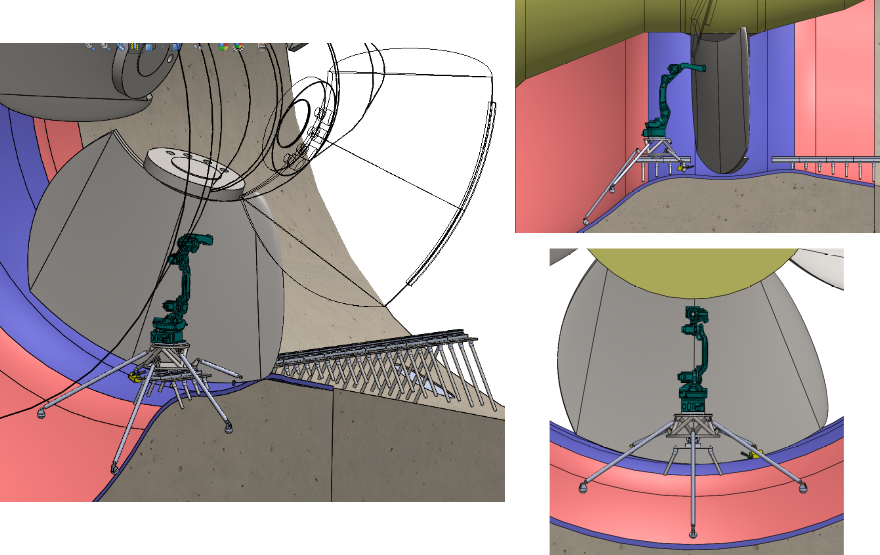
\includegraphics[width=0.8\columnwidth]{figs/bases/base_p}
   \caption{Base Prismática}
   \label{fig::base_p}
\end{figure}
  
  Este conceito foi estudado para o manipulador MH$12$, que de acordo com a
  análise cinemática consegue processar toda a extensão vertical. Para outros
  manipuladores, seria necessário incluir uma junta prismática, adicionando um
  grau de liberdade, na direção vertical.
  
  A análise cinemática também demonstrou que seriam necessárias muitas posições
  do rotor para completar uma face da pá. Há inclusive dificuldades operacionais e
  de segurança no procedimento de rotação do rotor que devem ser considerados. O
  rotor só pode ser girado manualmente, não fornecendo precisão no
  posicionamento da pá em relação a base. Por ser uma tarefa manual, deve-se ter
  procedimentos adequados de segurança para preservar tanto o operador quanto os
  equipamentos próximos. Estas preocupações tornam a solução pouco prática sob o
  ponto de vista operacional.

$\bullet$~\textbf{Base Prismática-Rotacional-Prismática (P-R-P):}

  Este conceito consiste de uma base composta por um trilho primário (junta
  prismática $1$), uma plataforma de base pivotada por mancal e rolamentos entre
  o trilho primário e secundário (junta rotacional) e um trilho secundário
  (junta prismática $2$). Montado o trilho primário alinhado ao eixo da turbina
  a base rotacional sobre o trilho primário, fixa-se o robo sobre a base
  rotacional. Esta base permitrá a montagem do trilho secundário apenas quando o
  robô atingir a região de interesse para revestimento. Quando posicionado o
  manipulador, monta-se então o trilho secundário alinhado ao plano paralelo a
  face da pá e ancora-se a base no ambiente. Desta forma, o robô pode-se
  movimentar ao longo de toda a extensão da pá por meio do trilho secundário e
  também se aproximar e se afastar da superfície da pá, por meio do trilho
  primário. A figura~\ref{fig::base_prp} ilustra este conceito.

\begin{figure}[h!]
   \centering
   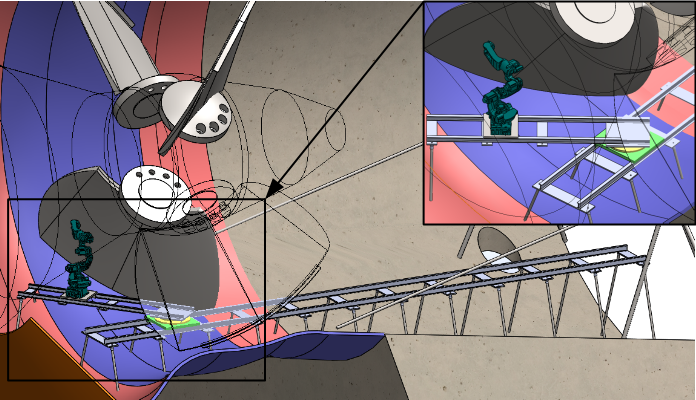
\includegraphics[width=0.9\columnwidth]{figs/bases/base_prp}
   \caption{Base Primática-Rotacional-Prismática}
   \label{fig::base_prp}
\end{figure}

  Desta forma, o rotor deve estar girado em, no mínimo $30^o$ para não haver
  contato com o trilho primário. A análise cinemática será realizada para
  encontrar a melhor configuração de juntas da base que permite ao robô se
  movimentar nos graus de liberdade da base, sem alterar o posicionamento do
  rotor e, assim, cobrir uma face inteira da pá. Para a repetição do processo
  nas outras pás do lado da sucção da turbina, é necessária a desmontagem do
  trilho secundário, o recuo do robô e desmontagem de parte do trilho primário,
  permitindo o giro do rotor para a pá seguinte.
  Para as faces do lado de adução, não é necessária a desmontagem parcial do
  trilho primário.
  
\subsection{Sistemas de elevação, fixação e ancoragem}
A entrada de pessoal através da escotilha é feita por uma escada vertical com
guarda-corpo com uma altura total de $5~m$. Equipamentos de segurança como
cinto e talabarte devem ser usados para qualquer um que deseja entrar no
ambiente confinado da turbina, através da escada e isso impossibilita o
transporte manual dos equipamentos. Por este motivo, deve ser instalada uma
estrutura com talha que permita a elevação até o interior da turbina e
movimentação para a áera de montagem adequada. As figuras~\ref{fig::talha} e
\ref{fig::talha_trilho} ilustram a estrutura de elevação com talha e carro
trole. 
  
\begin{figure}[h!]
   \centering
   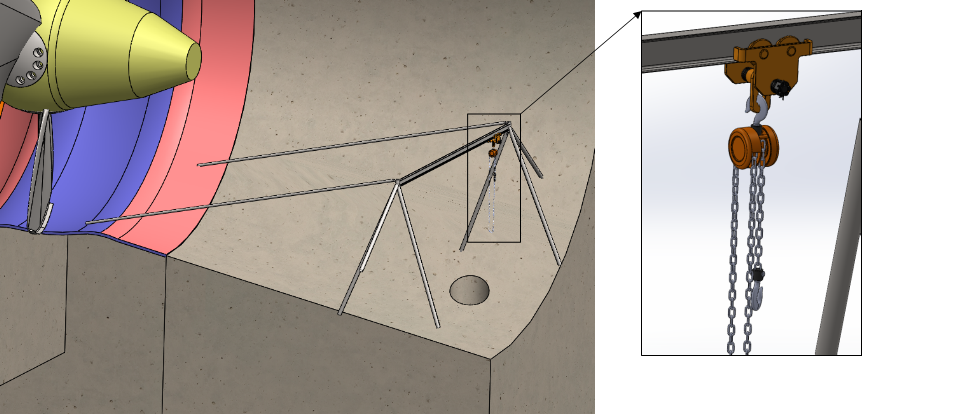
\includegraphics[width=0.8\columnwidth]{figs/bases/talha}
   \caption{Sistema de elevação dos equipamentos}
   \label{fig::talha}
\end{figure}

\begin{figure}[h!]
   \centering
   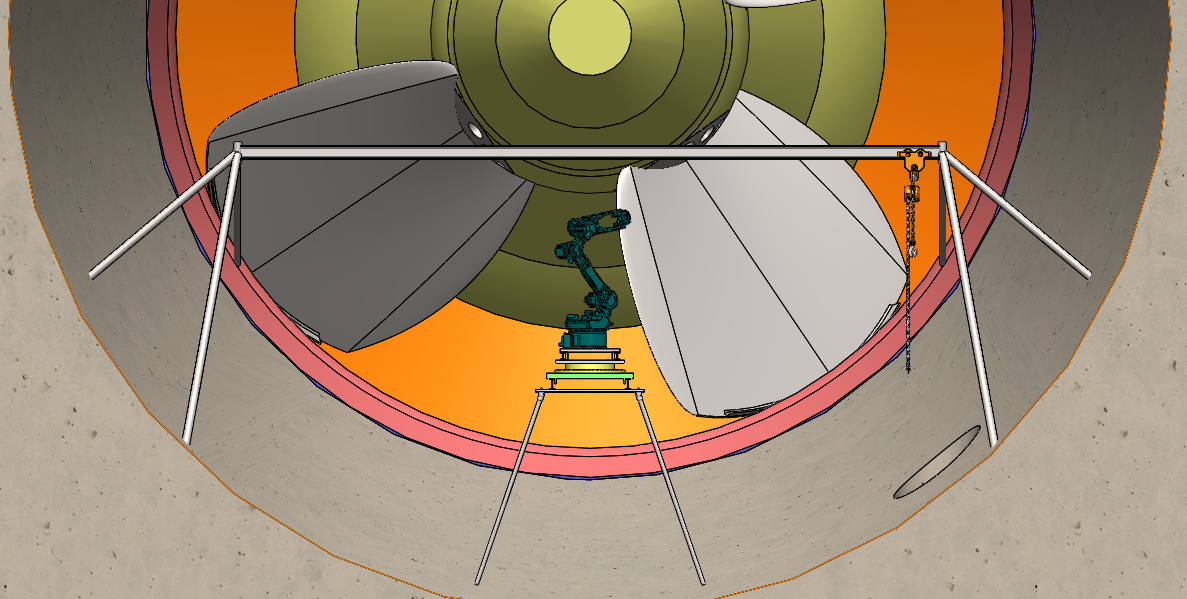
\includegraphics[width=0.8\columnwidth]{figs/bases/talha_trilho}
   \caption{Visão frontal da talha e trilho}
   \label{fig::talha_trilho}
\end{figure}

Devido aos esforços dinâmicos de operação do robô, a fixação da estutura da
base mecânica no ambiente deve ser dimensionada com cuidado. Por se
tratar de um ambiente de escoamento de fluido sob pressão, não são admitidas
modificações permanentes de infra-estrutura no interior da turbina, logo,
qualquer método de fixação utlizado deve ser removível, sem causar nenhum dano
à qualquer superfície. Em visita técnica realizada em Outrubro de $2015$ foi
testada a viabilidade de utlização de bases magnéticas para o sistema de
ancoragem e fixação. Este teste teve o objetivo de verificar a real carga limite de tração
do imã, considerando o ambiente (geometria), materiais e acabamentos
superficiais reais a que estará submetido na solução final. O resultado
detalhado do teste encontra-se no Apêndice~\ref{ape::magnetic}.

Outra opção para fixação provisória seria a soldagem da estrutura na
superfície do túnel. Esta opção segue como uma alternativa ainda para regiões
de difícil fixação da base magnética.
  
\subsection{Shutter}%TODO mudar o nome do sistema de desvio do fluxo de
% revestimento
O processo de revestimento HVOF (\textit{High Velocity Oxygen Fuel}) requer
velocidade da pistola controlada de $40~m/min$. Esta velocidade é essencial para
a qualidade do processo e deve ser mantida constante para se obter uma camada 
regular de material ao longo de toda a superfície da peça. Na solução
pesquisada demonstou-se ser inviável utilizar um robô de grande porte, devido a
limitação de acesso e ao confinamento do manipulador no ambiente. Portanto, o
manipulador  escolhido realizará o processo em regiões delimitadas da
superfície da peça e na trajetória haverá inevitavelmente mudanças de direção e
portanto acelerações que irão variar a velocidade da pistola. Durante essas
variações não deve-se injetar o material na peça, sendo necessário um mecanismo
autônomo para impedir o processo nestes intervalos.

A ideia inicialmente estudada foi de uma barreira ao fluxo na saída da pistola. 
A figura~\ref{fig::shutter_todos} ilustra a ideia para dois conceitos nas
configurações aberta e fechada. 
Nestes conceitos, uma barreira é movimentada automaticamente sempre que houver
mudança de direção da pistola, impedindo que o fluxo de material atinja a
pistola. 

\begin{figure}[h!]
   \centering
   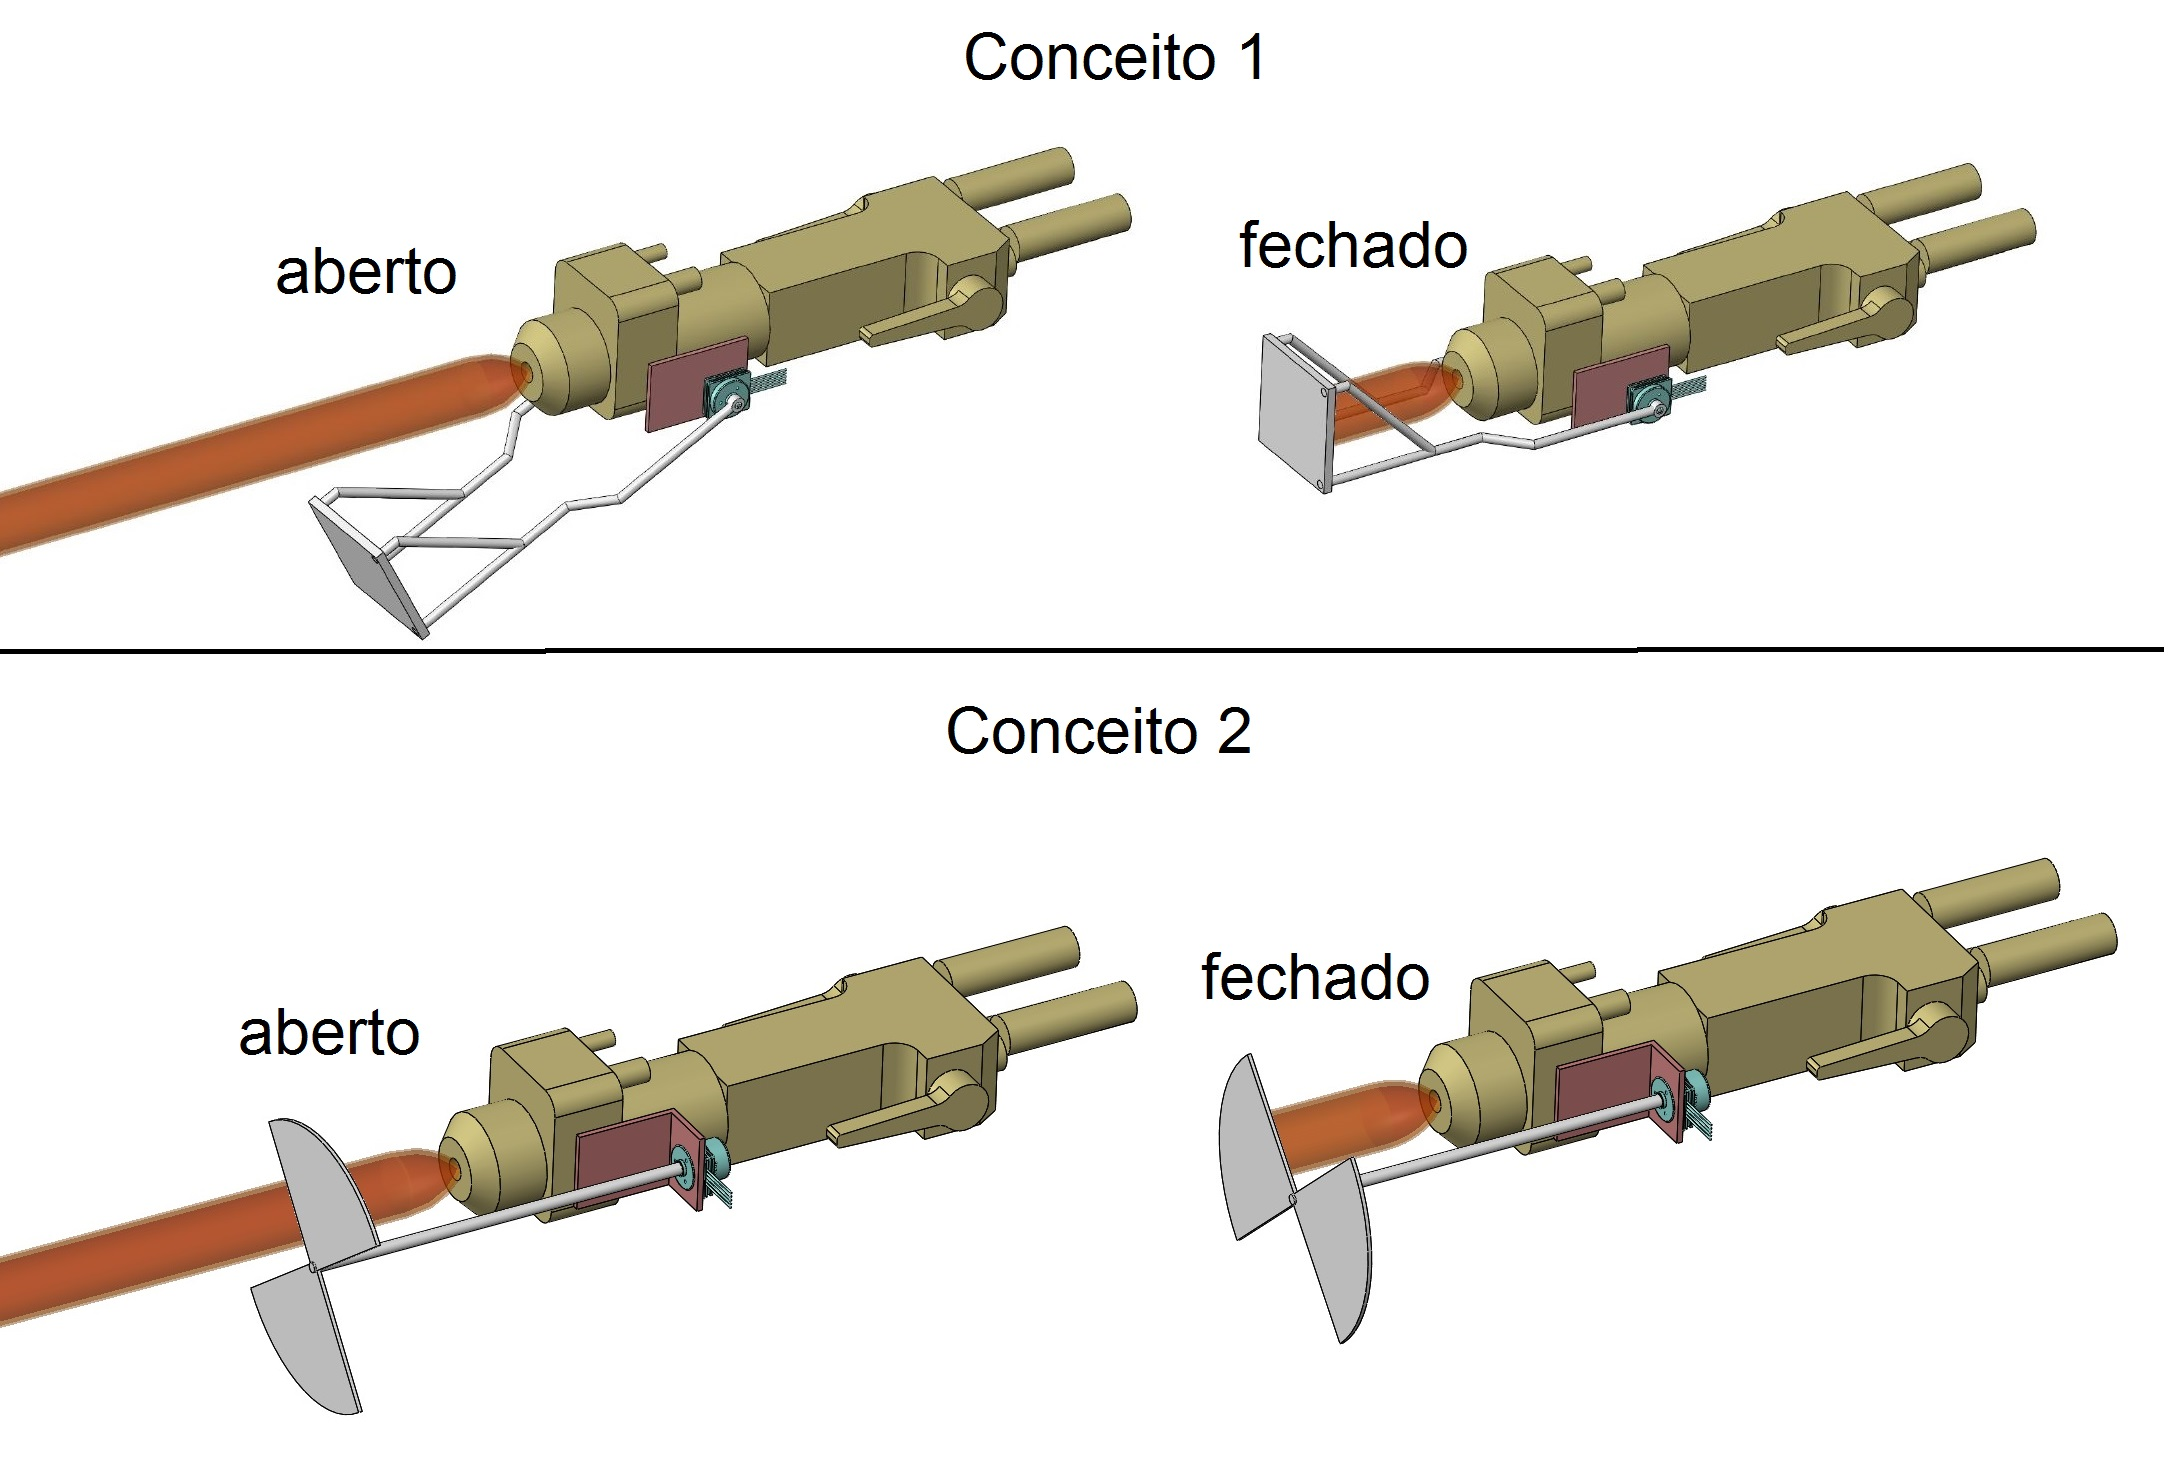
\includegraphics[width=0.8\columnwidth]{figs/shutter/shutter_todos}
   \caption{Conceitos de Shutter avaliados}
   \label{fig::shutter_todos}
\end{figure}

Algumas considerações foram levantadas para avaliar a viabilidade
desta solução, como a alta temperatura da chama, a capacidade do atuador, a
resistência mecânica da barreira e a taxa de acúmulo de material. Este conceito
foi abandonado principalmente devido ao acúmulo de material na barreira, o que
levaria a um aumento de seu peso e por consequência momento de inércia,
alterando a dinâmica prevista ou ainda poderia chegar a obstruir a saída da
chama, causando danos à pistola.

Outra proposta que está sendo estudada é a de modificar o fluxo da linha de
revestimento. A ideia é a inclusão de uma válvula direcional com atuação por
solenóide para desviar o fluxo do material de revestimento para um tanque ou
cilindro de retorno. Esta atuação deve ser autônoma assim como a
trajetória do manipulador. A válvula seria de três vias e duas posições ($3/2$) tal que, no 
repouso, direciona-se o fluxo diretamente para a pistola e, quando
atuada, bloqueia-se o fluxo para a pistola e abre-se o fluxo para exaustão. Uma
válvula limitadora de pressão regulável seria utilizada na linha de exaustão
para igualar as diferenças de pressão entre as duas vias, minimizando efeitos transitórios.
A figura~\ref{fig::circuito_hvof} apresenta o circuito do processo HVOF de forma
simplificada.

 \begin{figure}[h!]
   \centering
   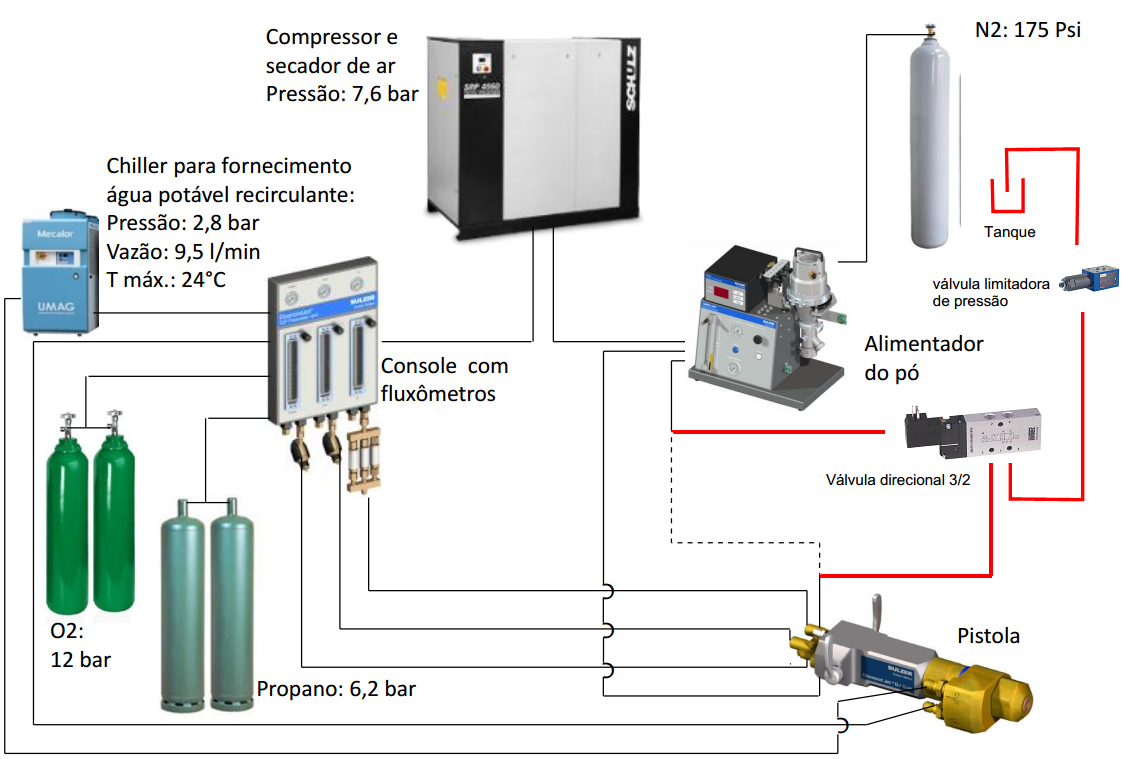
\includegraphics[width=0.8\columnwidth]{figs/shutter/Circuito_HVOF_mod}
   \caption{Circuito do processo HVOF modificado}
   \label{fig::circuito_hvof}
\end{figure}

A linha tracejada representa o circuito original, as linhas em vermelho
representam a modificação do circuito com os equipamentos adicionais indicados.

Esta é uma alternativa que tem como principal vantagem a de poder retornar a
matéria-prima do revestimento para tanque, ou seja, evita-se
o desperdício do material no ambiente. Esta matéria-prima poderia então ser
reaproveitada no processo, separando-se o gás.
